% coding:utf-8

%E-Wall
%Copyright (C) 2013, Daniel Winz, Ervin Mazlagic

%This program is free software; you can redistribute it and/or
%modify it under the terms of the GNU General Public License
%as published by the Free Software Foundation; either version 2
%of the License, or (at your option) any later version.

%This program is distributed in the hope that it will be useful,
%but WITHOUT ANY WARRANTY; without even the implied warranty of
%MERCHANTABILITY or FITNESS FOR A PARTICULAR PURPOSE.  See the
%GNU General Public License for more details.
%----------------------------------------

\section{Übersicht}

\subsection{Konzept}
Die Erkennung von Personen erfolgt mittels Ultraschall. Dabei wird die Laufzeit 
eines Signals gemessen und daraus die Anwesenheit von Personen bestimmt. Wird 
eine Person erkannt, wird das mit Lüftern und LEDs angezeigt. Die Steuerung 
übernimmt ein Mikrokontroller. 

\subsection{Aufbau / Blockschaltbild}
\begin{center}
\tikzstyle{block} = [ draw,fill=gray!20,text width=8em,align=center,
                      rounded corners,minimum height=5em]
\def\radius{.7mm}
\tikzstyle{branch}=[fill,shape=circle,minimum size=3pt,inner sep=0pt]
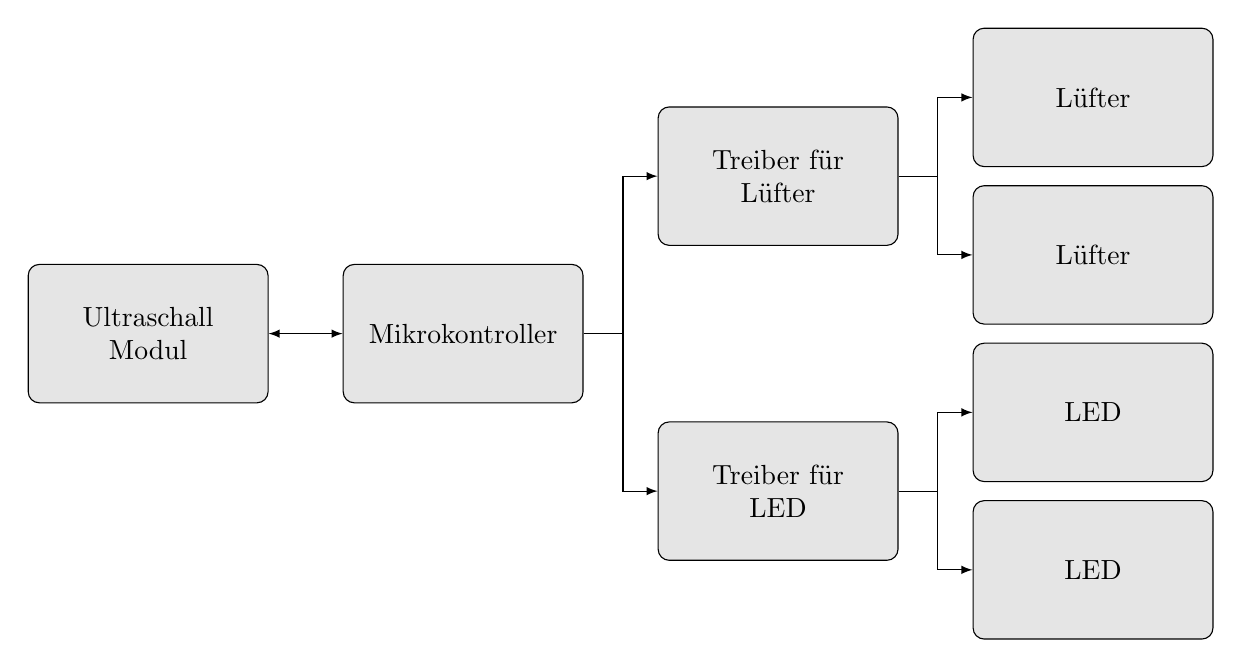
\begin{tikzpicture}
  \node[block] at (0,2) (us)   {Ultraschall \\ Modul};
  \node[block] at (4,2) (uc)   {Mikrokontroller};
  \node[block] at (8,0) (led)  {Treiber für \\ LED};
  \node[block] at (8,4) (fan)  {Treiber für \\ Lüfter};
  \node[block] at (12,1) (led1)  {LED};
  \node[block] at (12,-1) (led2)  {LED};
  \node[block] at (12,3) (fan1)  {Lüfter};
  \node[block] at (12,5) (fan2)  {Lüfter};
  
  \draw[latex-latex] (us.east) -- (uc.west);
  \draw[-latex] (uc.east) -- +(0.5,0) |- (led.west);
  \draw[-latex] (uc.east) -- +(0.5,0) |- (fan.west);
  \draw[-latex] (led.east) -- +(0.5,0) |- (led1.west);
  \draw[-latex] (led.east) -- +(0.5,0) |- (led2.west);
  \draw[-latex] (fan.east) -- +(0.5,0) |- (fan1.west);
  \draw[-latex] (fan.east) -- +(0.5,0) |- (fan2.west);
\end{tikzpicture}
\end{center}
